\documentclass[12pt,a4paper]{article}
\usepackage[utf8]{inputenc}
\usepackage[francais]{babel}
\usepackage[T1]{fontenc}
\usepackage{kpfonts}
\usepackage{pdfpages}
%\author{Mathieu Leocmach}
\title{Université de Tokyo}
\date{}
\begin{document}
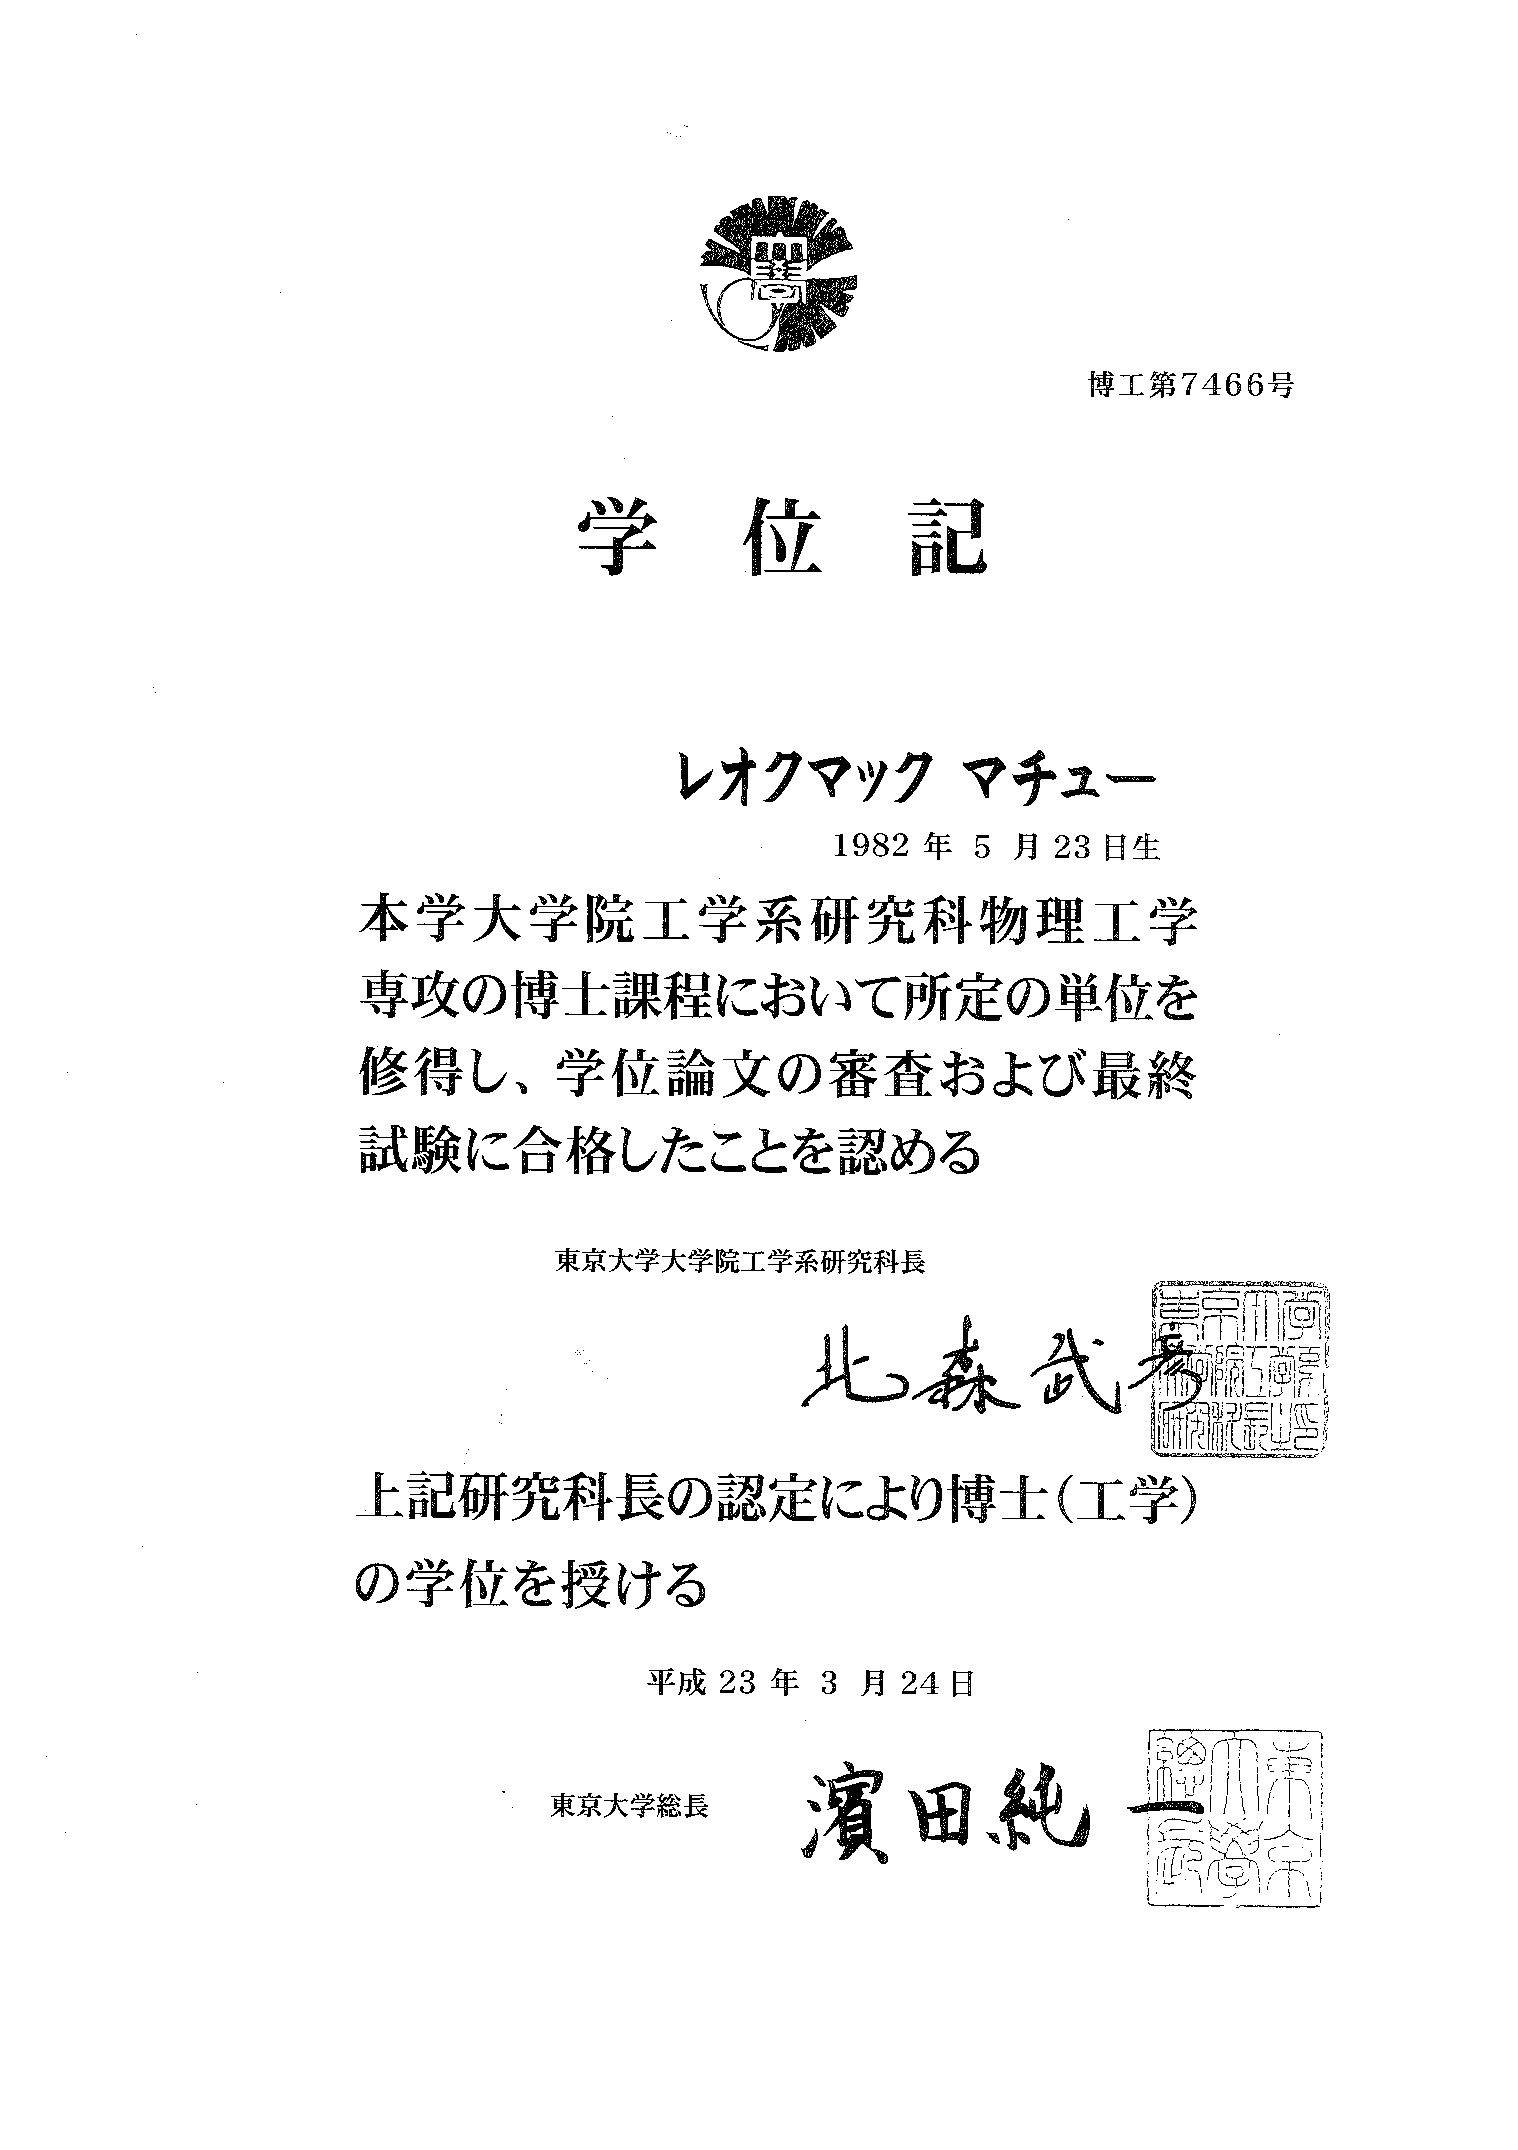
\includepdf[pages=-]{diplome_PhD.pdf}
\maketitle
\thispagestyle{empty}
\begin{center}

\textsc{Ce document atteste que la personne nommée ci-dessous a validé les unités nécessaires dans le troisième cycle de cette université, a réussi l'examen final et que la dissertation demandée a bien été acceptée par l'université.}

\bigskip

\textsc{Leocmach Mathieu\\
a été admis au grade de\\}
Docteur en ingénierie
\textsc{dans la spécialité\\
physique appliquée}
\end{center}

\bigskip

\begin{description}
\item[Date de naissance] 23 mai 1982
\item[Date du diplôme] 24 mars 2011
\item[Numéro du diplôme] HAKU KO 7466
\end{description}

\bigskip

Ceci est une transcription certifiée du diplôme en japonais.

\textit{Ceci est la traduction en français de la transcription certifié en anglais du diplôme en japonais}
\end{document}